% This is samplepaper.tex, a sample chapter demonstrating the
% LLNCS macro package for Springer Computer Science proceedings;
% Version 2.20 of 2017/10/04
%
\documentclass[runningheads]{llncs}
%
\usepackage{booktabs}
\usepackage{graphicx}
\usepackage{pgfplots}
\usepackage{tikz}
\usepackage{enumitem}
\usepackage{gensymb}
\usepackage{amsmath}
\usepgfplotslibrary{clickable}


\usepackage{listings}
\lstset{language=SQL,morekeywords={PREFIX,java,rdf,rdfs,url}}
% Used for displaying a sample figure. If possible, figure files should
% be included in EPS format.
%
% If you use the hyperref package, please uncomment the following line
% to display URLs in blue roman font according to Springer's eBook style:
% \renewcommand\UrlFont{\color{blue}\rmfamily}

\begin{document}
%
\title{Change estimation of SPARQL queries in Wikidata\thanks{Supported by CONICYT PFCHA/ DOCTORADO BECAS CHILE/2017 - 72180000 and Millennium Institute for Foundational Research on Data.}}
%
%\titlerunning{Abbreviated paper title}
% If the paper title is too long for the running head, you can set
% an abbreviated paper title here
%
\author{Alberto Moya\orcidID{0000-1111-2222-3333} \and
Aidan Hogan\orcidID{1111-2222-3333-4444} \and
Jesus P\'erez\orcidID{2222--3333-4444-5555} \and
Grethel Coello\orcidID{2222--3333-4444-5555}}
%
\authorrunning{A. Moya et al.}
% First names are abbreviated in the running head.
% If there are more than two authors, 'et al.' is used.
%
\institute{Computer Science Department, University of Chile, Chile\\
\email{\{amoya,ahogan,jperez,gcoello\}@dcc.uhile.cl}}
%
\maketitle              % typeset the header of the contribution
%
\begin{abstract}
Linked Open Datasets contain descriptions that change over time. The resources described by these datasets are continuously created, moved, deleted, linked, and unlinked. Applications that leverage Linked Data must be aware of these change dynamics to deliver accurate services. In this work, we tackle the problem of estimating future changes in query results based on query syntax features. We propose a model that exploits the characteristics of RDF to capture the dynamics of the predicates. Our Dynamics Model complements syntax features extracted from queries to assess if query results will change in the near future using classifiers and long future using Linear Regression. To evaluate our proposal, we select Wikidata as our dataset and we build a curated collection of queries. Our results show that the accuracy of our proposal approaches that obtained using information on the historical evolution of the query results but at a lower cost.

\keywords{Change estimation \and SPARQL query \and Link Data dynamics.}
\end{abstract}
%
%
	%
\section{Introduction}
\label{sec:intro}
%
The Linked Data (LD) principles\footnote{https://www.w3.org/DesignIssues/LinkedData.html} provide a flexible publishing paradigm to integrate and interlink data on the Web. Following the LD principles, a lot of organizations are publishing valuable information online using Resource Description Framework (RDF) and other LD technologies. The standardized approach to query these kinds of data is SPARQL, the recommendation of the W3C\footnote{https://www.w3.org/} to query RDF. There are many public SPARQL endpoints that allow any data consumer to query RDF datasets on the Web~\cite{VandenbusscheUM17}. Since the LD principles have been created, until now, the LOD cloud\footnote{https://lod-cloud.net/} has grown significantly~\cite{SchmachtenbergBP14}. 

Many applications that consume Linked Data face challenges related to changes in the underlying data, whose key is keeping data fresh. Since datasets change over time, long-running applications that cache and repeatedly use query results obtained from a SPARQL endpoint may resubmit the queries regularly to ensure up-to-dateness. As a result, applications often get the same results in several query executions, resulting in an unnecessary computation, and other times, they give the user stale results when the backend data change between re-executions. 

By caching the answers of queries and using the cached replies whenever possible, client-side caches reduce the network traffic between clients and servers, the load on servers, and the average user-perceived latency of query processing. However, for caches to be useful, cache consistency must be maintained, that is, cached copies should be updated when the data that gave rise to it change.
Ensuring a strong consistency in which no stale copy of the modified document will ever be returned to the user could be expensive. Thus, several weak consistency approaches have been proposed that try to keep the local data of the applications updated at lower cost~\cite{KnuthHS16,DividinoGS15,NishiokaS17}.

Some works have proposed to learn from historical entity evolution, but a query could involve many entities. Considering the historical evolution of all entities relating to a query is expensive because it is necessary to have the previous complete versions of data and to obtain the results of the execution of the query in each version. In addition, several recent works have explored the dynamics of the query results with the intention of finding patterns that allow for characterizing, recognizing, and predicting changes~\cite{KaferAUOH13,NishiokaS16,GonzalezH18}. Recent works have found some general correlations with datasets dynamics, such as, the domains, predicates, and schema~\cite{KaferAUOH13,NishiokaS17,UmbrichHHPD10}. Based on dynamic knowledge, hybrid approaches have been developed to return fresher results and at the same time speed up queries, but freshness estimates are a major and still current challenge, because of the difficulty of predicting the underlying dynamics on the growing Web of Data.

In this work, we tackle the problem of estimating future changes in query results based on data statistics and methods from Machine Learning. We devise a solution where we do not have complete information from the past, but a reduced statistical model that summarizes the historical dynamics based on predicates. Subsequently, we develop classifiers for assessing whether or not query results will change in the future. Additionally, we propose to use a set of features extracted from the query syntax.

We apply this framework to compute a predictive Dynamics Model for 23 versions of the Wikidata knowledge graph~\cite{VrandecicK14}, evaluating its suitability for predicting future changes in the query results. We select Wikidata as: (1) it provides a history of weekly versions that we can use to evaluate predictions and (2) it is edited by thousands of users, which means that significant changes are observed weekly. In addition, we build a dataset of real queries on Wikidata to monitor and to check the validity of our proposed approach. 

In summary, the \textbf{contributions} of this paper are: (i) we build a dataset of real queries for Wikidata, (ii) we provide an analysis of the evolution of the results of those queries over 23 weekly versions of Wikidata, (iii) we propose a classifier that judges whether or not the results of a query will change using a predicate-based Dynamics Model and features from the syntax of the query, and (iv) we show that the proposed features and classifier work well, and our results are close to the more expensive previous approaches that assume full knowledge of historical data.

The rest of this document is organized as follows: In Section~\ref{sec:related}, we review related works. Section~\ref{sec:preliminar} provides the formal definition of the problem. Section~\ref{sec:approach} describes our proposal. In Section~\ref{sec:data}, we explain our datasets. Section~\ref{sec:eval} presents the design and results of the experiments. We conclude and review future directions in Section~\ref{sec:conclusion}.


%
\section{Related Work}
\label{sec:related}
%

Many applications can benefit from change prediction in query results. Both, Smart Caching (to save computational resources) and Hybrid Architectures (to deliver fresh results in less time) require synchronization techniques. Several techniques have been developed following strong consistency, based on HTTP metadata~\cite{fielding2rfc} and notifications~\cite{PassantM10,Fitzpatrick10,TrampFEA10}. Other works seek weak consistency based on probabilities, such as Empirical Distributions~\cite{NeumaierU16}, Poisson Processes~\cite{UmbrichHHPD10}, and Markov Chains~\cite{UmbrichMP15}, as well as other works based on heuristics~\cite{AliciAOCU12,UmbrichMP15,KnuthHS16}, metrics~\cite{DividinoGS15,KnuthHS16,AkhtarAL17}, and Machine Learning~\cite{NishiokaS17,GonzalezH18}. In the case of metadata, some works~\cite{UmbrichHHPD10,DividinoKG14,Kjernsmo15,NeumaierU16} show that these data are often not provided or are wrong. In the case of notifications, several tools have been developed, such as rsine~\cite{MaderMS14} and Boca~RDF~\cite{MissierACDG07}, but these mechanisms must keep a subscriber list and open connection states that can also cause scalability problems. The rest of the approaches achieve interesting results, but the main deficiency in these approaches is that their quality depends on having a long and complete history of updates. In the case of ML-based approaches, they constitute a general framework where important improvements can be achieved by incorporating relevant features to the models. In our approach, we propose an ML-based solution that dispenses with the expensive history of updates by a lighter model with statistics from this history and syntactic query features.

Some works have tried to understand the dynamics of the LOD datasets~\cite{UmbrichHHPD10,UmbrichKL10,KaferAUOH13,DividinoSGG13,NishiokaS16}. Some features found to describe the dynamics of a resource are Pay-Level Domain (PLD)~\cite{NishiokaS16,NishiokaS17}, predicates~\cite{KaferAUOH13,NishiokaS17}, and Characteristic Sets (CS)~\cite{NishiokaS16,GonzalezH18} that are correlated with the dynamics of several datasets studied. This knowledge can be used to estimates the freshness of cached data. Umbrich et al.~\cite{UmbrichKHP12,UmbrichKPPH12,ekawUmbrichKHP12} identified two variants to obtain knowledge about freshness for different query patterns based on predicates. In more recent work Dehghanzadeh et al.~\cite{DehghanzadehPKUHD14} proposed a solution to estimate the freshness using cardinality estimation techniques based on predicates and CS. However, to the best of our knowledge, there is no proposal to estimate the freshness of cached query results using Machine Learning models based on syntactic features from queries and reduced historical statistics. In addition, the previous approaches usually impose restrictions on queries, such as not considering complex queries, e.g., with filters. Also, we do not find works that report the quality of the proposed models on complex real queries.


%
\section{Preliminaries: RDF and SPARQL}
\label{sec:preliminar}

According to the LD principles, the data published on the Web must be described using the Resource Description Framework (RDF). RDF is a conceptual model based on directed graphs that serves to provide descriptive information about the resources on the Web. The RDF nodes correspond to resources, literals (strings), or blank nodes, which model variables in the graph. Resources are identified by an Internationalized Resource Identifier (IRI). The nodes are linked through labeled and directed arcs, which represent semantic relationships.

\begin{definition}[RDF Triple and Dataset]
	Let I, L, and B be disjoint sets of IRIs, literals, and blank nodes respectively. A tuple $ (s, p, o) \in (I \cup  B)  \times (I)  \times  (I \cup  B \cup  L)$  is called an RDF $ triple $, where $ s $ is called subject, $ p $ is called predicate, and $ o $ is called object. An RDF $dataset$ is a set of RDF $triples$.
\end{definition}

SPARQL is the recommended query language to retrieve and manipulate data stored in the RDF format. In this work, we focus on SPARQL SELECT queries, which return the set of variables and their mapping results. Here we define a SPARQL 1.0 query. 

\begin{definition}[SPARQL expression]
	Let V be a set of variables disjoint from $U \cup B \cup L$. A SPARQL $expression$ is built recursively as follows. (1) A triple $pattern t \in  (U \cup V ) \times (U \cup V ) \times (L \cup U \cup V )$ is an $expression$. (2) If $Q_1$ and $Q_2$ are $expressions$ and R is a filter condition, then $Q_1$ FILTER R, $Q_1$ UNION $Q_2$, $Q_1$ OPTIONAL $Q_2$, $Q_1$ AND $Q_2$ are $expressions$.
\end{definition}

A triple $ pattern $ in the second position can contain an expression called \textit{Property Paths} since SPARQL~1.1 to allow for navigational querying over RDF graphs. Other features at SPARQL~1.1 will be seen in experiments.

\begin{definition}[Property Paths]
	\label{eq:pp}
	Property Paths expressions are defined by the grammar:\\
	
	\begin{tabular}{ll}    \hline
		Rules &  \\    \hline
		e $\rightarrow$ p & a predicate \\
		
		e $\rightarrow$ \^{}e    &  inverse path \\
		
		e $\rightarrow$ e $/$ e    &  a path of $ e_1 $ followed by $ e_2 $\\
		
		e $\rightarrow$ e $\mid$ e    &  a path of $ e_1 $ or $ e_2 $ \\
		
		e $\rightarrow$ e*    &  a path of zero or more $ e $ \\
		
		e $\rightarrow$ e+    &  a path of one or more $ e $ \\
		
		e $\rightarrow$ e?    &  a path of zero or one $ e $ \\
		
		e $\rightarrow$ !p    &  any predicate not $ p $ \\
		
		e $\rightarrow$ !( p1,...,pk, \^{}p1,...,\^{}pk)    &  any (inverse) predicate not listed \\
		
		e $\rightarrow$ ( e )    &  brackets used for grouping \\    \hline
	\end{tabular}
	
	where $p, p1,...,pk$ are IRIs in $I$.
\end{definition}

\section{Our Approach}
\label{sec:approach}

Next, we formalize the problem addressed in this work and present our proposed solution.

\subsection{Problem Definition and Proposed Solution}

For this work, we consider a dynamic RDF dataset, denoted by $\mathcal{D}$. In addition, we assume that we have consecutive sequence of $m$ past versions $\mathcal{D} = (d_1, d_2, ..., d_m)$ constituting different revisions fetched at regular intervals. We also consider a SPARQL SELECT query $q$, of which we would like to know if its results are going to be valid for a long time. For that, we have the results of $q$ on each of the $m$ past versions of $\mathcal{D}$ and we need to know when we should update it. Then, we call $q(d_i)$ the result of executing the query $q$ on the $d_i$ version of $\mathcal{D}$.\\

In addition, we consider delta ($\delta$) a function to compute the binary dissimilarity between two results for a query $q$ with the following expression:

\begin{equation}
\label{eq:delta}
\delta(q(d_i), q(d_j)) = \begin{cases}
0 & q(d_i) = q(d_j) \\
1 & q(d_i) \neq q(d_j) 
\end{cases}
\end{equation}

\begin{example}
	\label{ex:dataset}    
	Consider the following examples of seven versions of a dynamic RDF dataset that contains a subject and four properties. Also, consider the queries~\ref{lst:sparql0}, \ref{lst:sparql1} and \ref{lst:sparql2}.
\end{example}

\setlength{\tabcolsep}{6pt}
\begin{tabular}{l l l}    \hline	
	\multicolumn{3}{c}{versions $d_1$ and $d_2$} \\    \hline
	:Atlantic\_Ocean  & :instance\_of  & ocean          \\
	:Atlantic\_Ocean  & :temperature   & 40$\degree$F          \\
	:Atlantic\_Ocean  & :area          & $10^7\pm10^3$ $km^2$ \\
	:Atlantic\_Ocean  & :image         & AOcean1.png    \\    \hline
	\multicolumn{3}{c}{versions $d_3$, $d_4$ and $d_5$} \\    \hline
	:Atlantic\_Ocean  & :instance\_of  & ocean          \\
	:Atlantic\_Ocean  & :temperature   & 50$\degree$F             \\
	:Atlantic\_Ocean  & :area          & $10^7\pm10^3$ $km^2$ \\
	:Atlantic\_Ocean  & :image         & AOcean1.png    \\    \hline
	\multicolumn{3}{c}{versions $d_6$ and $d_7$} \\    \hline
	:Atlantic\_Ocean  & :instance\_of  & ocean          \\
	:Atlantic\_Ocean  & :temperature   & 60$\degree$F    \\
	:Atlantic\_Ocean  & :area          & $10^7\pm10^3$ $km^2$ \\
	:Atlantic\_Ocean  & :image         & AOcean1.png    \\
	:Atlantic\_Ocean  & :image         & AOcean2.png    \\    \hline
\end{tabular}\\

\begin{lstlisting}[captionpos=b, caption=SPARQL query about ocean temperatures., label=lst:sparql0,
basicstyle=\ttfamily,frame=single]
SELECT ?ocean ?temp
WHERE {
  ?ocean :instance_of :ocean .
  ?ocean :temperature ?temp
}
\end{lstlisting}

\begin{lstlisting}[captionpos=b, caption=SPARQL query about ocean areas., label=lst:sparql1,
basicstyle=\ttfamily,frame=single]
SELECT ?ocean ?area
WHERE {
  ?ocean :instance_of :ocean .
  ?ocean :area ?area
}
\end{lstlisting}

\begin{lstlisting}[captionpos=b, caption=SPARQL query about ocean images., label=lst:sparql2,
basicstyle=\ttfamily,frame=single]
SELECT ?ocean ?image
WHERE {
?ocean :instance_of :ocean .
?ocean :image ?image
}
\end{lstlisting}

$\delta(q_1(d_1), q_1(d_3)) = 1$ and $\delta(q_2(d_2), q_2(d_4)) = 0$

Based on the $\delta$ function (see Equation~\ref{eq:delta}), the problem of Time-to-Live (TTL) estimation, denoted by $TTL(q,m)$ is defined by the size of the largest interval from $m$ for which the query result does not change (see Equation~\ref{eq:ttl}).

\begin{equation}
\label{eq:ttl}
TTL(q,m)=min\{t \in \mathbf{Z}^+ \mid \delta(q(d_m), q(d_{m+t})) \neq 0 \}
\end{equation}

As a relaxed version of this problem, there is the problem of One-Step-Change (OSC) estimation to predict the change in the next interval. (see Equation~\ref{eq:osc})

\begin{equation}
\label{eq:osc}
OSC(q,m) = \delta(q(d_m), q(d_{m+1}))
\end{equation}

Considering the dataset from Example~\ref{ex:dataset} and queries~\ref{lst:sparql0}, \ref{lst:sparql1} and \ref{lst:sparql2}, we show the change history of the query $q_1$ (see Figure~\ref{fig:problem}). We mark with a discontinuous line the OSC and with a continuous line the TTL at version $ d_3 $. The OSC is equal to zero, which means that the results will not change in the next version $d_4$, and the TTL equals three.

\begin{figure}[h]
	\centering
	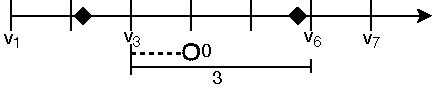
\includegraphics[width=0.7\linewidth]{img/problem.pdf}
	\caption{Example change history of query $q_1$.}
	\label{fig:problem}
\end{figure}

We propose a scheme that automatically identifies whether a SPARQL query will change in the next version (OSC) or when it will change (TTL), depending on the syntax of the query and statistics about the dynamics of predicates. Figure~\ref{fig:schema} shows the components of our approach, which receives as input a SPARQL query. The Feature Extractor analyzes the query and extracts information about the syntax of the query. The Dynamics Model considers some of these features to provide a dynamics indicator of the query. This indicator, together with the previous features extracted, is passed through a classifier that finally predicts the value for the problems posed in Equation~\ref{eq:osc} and Equation~\ref{eq:ttl}.

\begin{figure*}[!ht]
	\centering
	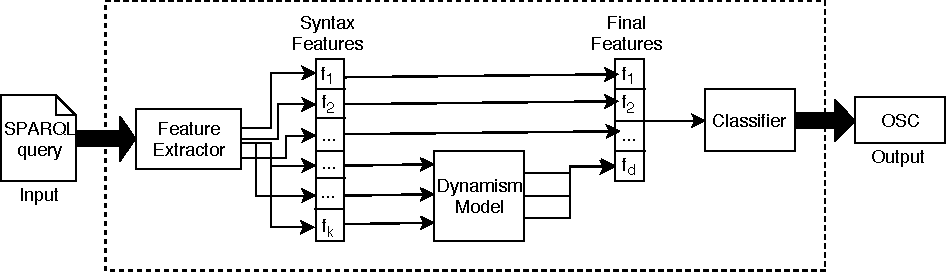
\includegraphics[width=0.7\linewidth]{img/schema.pdf}
	\caption{ Proposed architecture. It receives a SPARQL query as input; uses a pre-calculated Dynamics Model to estimate a query dynamic feature, which is used with other features to predict the OSC and TTL values. }
	\label{fig:schema}
\end{figure*}

\subsection{Feature Extractor}

In order to predict when the results of a query will change, we propose a framework based on Machine Learning using features extracted from the queries. Our features are based on the syntactic analysis of the queries; then some features are delivered to the Dynamics Model, which provides an indicator based on the probability of change for the constant predicates within the triple patterns of the query.

The extracted features try to capture the basic characteristics of a query. We try to discover the degree of correlation between the propensity to change, with respect to numerical values, such as the number of variables, the number of triple patterns, the number of predicate or entity constants, or the number of projected variables. We also believe that some qualitative variables may be related to the change, such as the existence of some solution-modifiers.

We also consider features that describe the complexity of the queries, such as the presence of subqueries, the existence of recursive expressions in the Property Paths of the triple patterns or the existence of any type of negation.

Figure~\ref{fig:query} shows the complete list of evaluated features and shows the nominals. In the case of negation, we consider the statements MINUS, FILTER NOT EXISTS, and FILTER NOT BOUND and by the recursive path we understand those Property Paths that have patterns of the form $e*$ or $e+$ (see Definition~\ref{eq:pp}).

\begin{lstlisting}[captionpos=b, caption=Query example, label=fig:query,
basicstyle=\ttfamily,frame=single]
SELECT ?item
WHERE {
  ?item :instance_of :human .
  ?item :gender :female .
    { ?item :place_of_birth :Wales }
  UNION
    { ?item :place_of_birth ?pob .
      ?pob :located_in* :Wales }
  OPTIONAL { ?sitelink schema:about ?item .
             ?sitelink schema:inLanguage "cy" }
  FILTER (!BOUND(?sitelink))
}
LIMIT 100
\end{lstlisting}

\begin{center}
	\begin{tabular}{|l|ll|}    \hline
		1  & \# triples        & 7                             \\
		2  & \# vars           & 3                             \\
		3  & \# projected vars & 1                             \\
		4  & \# predicates     & 6                             \\
		5  & FILTER            & TRUE                          \\
		6  & LIMIT             & TRUE                          \\
		7  & UNION             & TRUE                          \\
		8  & SUBQUERY          & FALSE                         \\
		9  & *PATH             & TRUE                          \\
		10 & NEGATION          & TRUE                          \\
		11 & predicates        & {[}$p_1$,...,$p_k${]}    \\    \hline
	\end{tabular}
\end{center}



\subsection{RDF Dynamics Model}

We propose a model to estimate the dynamics of the results of a SPARQL query on an RDF dataset. The intuition behind our model is to capture how many triples change for a predicate in a time interval. For this, in the following, we define \textit{Predicate Multiplicity of an RDF dataset}.

\begin{definition}[Predicate Multiplicity of an RDF Dataset]
	Given an RDF dataset $d$ and a predicate $p$, the multiplicity of $p$ in $d$, denoted by $M(p,d)$, is:
	\begin{equation}
	\label{eq:pm}
	M(p,d) = |\{(x,y,z) \in d : y = p \}|
	\end{equation}
\end{definition}


\begin{example}
	\label{ex:pm}    
	Considering Example~\ref{ex:dataset}, the Predicate Multiplicity of predicate \textit{image} in $d_6$ dataset is:    $M(image,d_6) = 2$
\end{example}


Then, we must capture the change between two versions of an RDF dataset at the triples level, which represents triples added and deleted between the versions. For this purpose, we define a \textit{Difference Set} as an RDF dataset denoted by $\Delta(d_1, d_2)$ applying low-level change detection techniques.

\begin{definition}[Difference Set]
	Let $d_1$ and $d_2$ be two RDF datasets; a Difference Set denoted by $\Delta(d_1, d_2)$ is:
	\begin{equation}
	\label{eq:ds}
	\Delta(d_1, d_2) = \{t \mid t \in d_2 \wedge t \notin d_1\} \cup \{t \mid t \in d_1 \wedge t \notin d_2\}
	\end{equation}
\end{definition}

\begin{example}
	\label{ex:ds}
	We show the Difference Set between versions $d_1$ and $d_6$:\\
	\begin{center}    
		\begin{tabular}{lll}    \hline
			\multicolumn{3}{c}{$\Delta(d_1, d_6)$} \\    \hline
			-    :Atlantic\_Ocean  & :temperature   & 40$\degree$F          \\
			+    :Atlantic\_Ocean  & :temperature   & 60$\degree$F          \\
			+    :Atlantic\_Ocean  & :image         & AOcean2.png              \\    \hline
		\end{tabular}
	\end{center}
	
	We can now denote the Predicate Multiplicity of a Difference Set of $d_1$ and $d_2$ by $M(p, \Delta(d_1, d_2))$, e.g., $M(image, \Delta(d_1, d_6)) = 1$.
\end{example}


Following the intuition of our model, we now look for the multiplicity of a predicate $p$ of a dynamic dataset $\mathcal{D}$ in a time interval $[n,m]$.

\begin{definition}[Aggregated Predicate Multiplicity of a dynamic dataset]
	Let $\mathcal{D} = (d_1, d_2, ..., d_m)$ be a dynamic dataset, and $p$ a predicate. The Aggregated Predicate Multiplicity of $\mathcal{D}$ in a time interval $[n,m]$, denoted by $AM(p, \mathcal{D},[n,m])$ is:
	\begin{equation}
	\label{eq:apm}
	AM(p, \mathcal{D},[n,m]) = \sum_{i=n}^{m-1}M(p, \Delta(d_i, d_{i+1}))
	\end{equation}
\end{definition}

\begin{example}
	\label{ex:apm}
	$AM(temperature, \mathcal{D},[1, 7]) =$
	
	$ \sum_{i=1}^{6}M(temperature, \Delta(d_i, d_{i+1})) = 4$
	
	\begin{center}    
		\begin{tabular}{lll}    \hline
			\multicolumn{3}{c}{$\sum_{i=1}^{6}\Delta(d_i, d_{i+1})$} \\    \hline
			-    :Atlantic\_Ocean  & :temperature   & 40$\degree$F          \\
			+    :Atlantic\_Ocean  & :temperature   & 50$\degree$F          \\            
			-    :Atlantic\_Ocean  & :temperature   & 50$\degree$F          \\
			+    :Atlantic\_Ocean  & :temperature   & 60$\degree$F          \\
			+    :Atlantic\_Ocean  & :image         & AOcean2.png              \\    \hline
		\end{tabular}
	\end{center}
\end{example}

We can now denote the Aggregated Multiplicity of a dynamic dataset in a time interval $[n,m]$ by:

\begin{equation}
\label{eq:am}
AM(\mathcal{D},[n,m]) = \sum_{p \in P}AM(p, \mathcal{D},[n,m])
\end{equation}\\
Where $ P $ denotes the set of all predicates that have changed in the interval $[n,m]$.

\begin{example}
	\label{ex:am}
	$AM(\mathcal{D},[1,7]) = AM(temperature, \mathcal{D},[1,7])$
	
	$+ AM(image, \mathcal{D},[1,7]) = 5$
\end{example}

Finally, the \textit{Dynamics} of a predicate is given by the \textit{Aggregated Predicate Multiplicity of a dynamic dataset} $\mathcal{D}$ divided by \textit{Aggregated Multiplicity of a dynamic dataset}.

\begin{equation}
\label{eq:dyn}
Dyn(p, \mathcal{D},[n,m]) = \frac{AM(p, \mathcal{D},[n,m])}{AM(\mathcal{D},[n,m])}
\end{equation}

\begin{example}
	\label{ex:dyn}
	Considering our example:
	
	$ Dyn(temperature, \mathcal{D},[1,7]) = \frac{4}{5} = 0.8$
	
	$ Dyn(image, \mathcal{D},[1,7]) = \frac{1}{5} = 0.2$
	
	$ Dyn(area, \mathcal{D},[1,7]) = \frac{0}{5} = 0$
\end{example}

Considering our proposed model, the Dynamics Model component receives the set of predicates extracted from the queries, calculates the $Dyn(p, \mathcal{D},[n,m])$ for each predicate $p$ and provides the value of a Transformation Function on these indicators. The idea behind the Transformation Function is to estimate the dynamics of the query based on the Dynamics of the predicates, e.g., Average and Maximum.


\section{Datasets}
\label{sec:data}

We conducted an empirical study to evaluate the effectiveness of our proposal to predict change in SPARQL query results. For this, we need an RDF dataset, with a lot of information, preferably, cross-domain, and that is constantly updated since we assume that the information of the dataset is correct, complete, but dynamic. We also need a set of queries appropriate to the chosen dataset, preferably a heterogeneous set defined by real users and covering a large part of the dataset.

\subsection{RDF Dataset}

We use Wikidata as one of the largest cross-domain knowledge graphs. There are several different kinds of data dumps available in JSON, XML, and RDF formats. We use 23 snapshots from 18/04/2017 to 27/09/2017, which are captured weekly. We worked with the truthy version in the RDF N-triples format, which represents statements that have the best non-deprecated rank for a given property.

The first version has 1,102,242,331 triples, 57,499,191 unique IRIs, 3,276 unique predicates, 933,588,860 literals, and 7,449 blank nodes, while the final version has 1,924,967,162 triples (+74\%), 80,637,164 unique IRIs (+40\%), 3,660 unique predicates (+11\%), 1,676,930,476 literals (+79\%) and 8,909 blank nodes (+19\%). Wikidata is maintained collaboratively by volunteer editors. Figure~\ref{graph:datasize} shows the growth maintained over the period of some of these indicators. The gap in week 12 is due to the fact that we were not able to obtain the data for that week. Even though the information is relatively incremental, there are deletions. Figure~\ref{graph:delta} shows the ratio of triples eliminated and added each week.

\begin{figure}[h]
	\begin{minipage}[b]{0.40\linewidth}
		\centering
		\begin{tikzpicture}[thick, scale=0.5]
		\begin{axis}[
		%title={Temperature dependence of CuSO$_4\cdot$5H$_2$O solubility},
		xlabel={Version},
		ymin=0,
		xtick={0,5,10,15,20,25},
		legend pos=north west,
		ymajorgrids=true,
		grid style=dashed,
		]
		
		\addplot[
		color=blue,
		mark=square,
		]
		coordinates {
			(1,1102242331)(2,1138975810)(3,1141303957)(4,1170283653)(5,1176093821)(6,1184177503)(7,1190456714)(8,1211813217)(9,1239145151)(10,1271353260)(11,1293099057)
		};
		
		\addplot[
		color=blue,
		mark=square,
		]
		coordinates {
			(13,1348622441)(14,1418460320)(15,1432143355)(16,1470298276)(17,1506140622)(18,1542278452)(19,1593334993)(20,1613832004)(21,1684774955)(22,1771601730)(23,1843086909)(24,1924967162)
		};
		
		%\legend{# entities}
		%\legend{# predicates}
		%\legend{# literals}
		%\legend{# blank nodes}
		
		\end{axis}
		\end{tikzpicture}
		\caption{Evolution of the number of triples on Wikidata.}
		\label{graph:datasize}
	\end{minipage}
	\hspace{0.5cm}
	\begin{minipage}[b]{0.40\linewidth}
		\centering
		\begin{tikzpicture}[thick, scale=0.5]
		\begin{axis}[
		x tick label style={
			/pgf/number format/1000 sep=},
		%ylabel=\#Triples,
		enlargelimits=0.05,
		legend style={at={(0.5,-0.1)},
			anchor=north,legend columns=-1},
		ybar interval=0.7,
		]
		\addplot 
		coordinates {(1,40137188)(2,4563382)(3,29302968)(4,8906402)(5,11455047)(6,11435682)(7,27229516)(8,26968577)(9,38952400)(10,20283316)(11,0)(12,0)(13,70073220)(14,17685830)(15,45405782)(16,41199256)(17,42633484)(18,56683899)(19,25309217)(20,25030143)(21,22548371)(22,23330356)(23,37009794)};
		\addplot 
		coordinates {(1,3403743)(2,2235268)(3,1116111)(4,3096270)(5,3371448)(6,5156519)(7,5873153)(8,1336452)(9,6744349)(10,999601)(11,0)(12,0)(13,1123311)(14,4002828)(15,7250907)(16,5356971)(17,6495717)(18,5627376)(19,4812243)(20,790590)(21,681118)(22,1194899)(23,998105)};
		\legend{Added, Removed}
		\end{axis}
		\end{tikzpicture}
		\caption{Triples added and removed in Wikidata.}
		\label{graph:delta}
	\end{minipage}
\end{figure}

\subsection{Queries Dataset}

Given our dynamic, cross-domain, large dataset, with historical information about its evolution, we now need a collection of queries for the dataset.

As opposed to RDF data, which can be easily obtained in the form of dumps, at the time of conducting this research, we did not find any structured dataset with queries following the Wikidata data model. Besides, Wikidata query logs are inaccessible, which would be interesting to understand the current usage of these data.

We found a set of 388 queries of examples about Wikidata\footnote{https://www.wikidata.org/wiki/Wikidata:SPARQL\_query\_service/queries/examples}, distributed in 18 categories. We consider these queries to evaluate our proposal. We crawled the sample queries from Wikidata in March 2018. This set is not a query log, but a wiki page containing selected queries sent by users. These queries are intended to show the behavior of the system or highlight the characteristics of the Wikidata dataset and, therefore, should reflect real-world queries.

Finally, the queries had to be curated manually, because they had syntax errors; others were not considered, because they asked information external to Wikidata, such as DBpedia\footnote{http://dbpedia.org/}, bigdata\footnote{http://www.bigdata.com/}; others asked for qualifiers that are not in the truthy version. We also eliminated the queries that returned bindings to blank nodes to facilitate the comparison between the results (they were only 10).

We consider query results as changed if it is not the same results returned for this query in the previous evaluation. Therefore, we need deterministic queries, that is, we remove those that could change their result even when the data is the same, such as, queries that contain the keyword SAMPLE and LIMIT without a total order. In our case, we eliminate the queries with the keyword SAMPLE and add ORDER BY to all the queries with all the projected variables. The latter change also facilitates the detection of changes in the results by iterating over both results sets in their sorted order.

Many queries use the custom Label service of Wikidata\footnote{https://www.mediawiki.org/wiki/Wikidata\_Query\_Service/User\_Manual\#Label\_service}. The service is very helpful when you want to retrieve labels, as it reduces the complexity of SPARQL queries that would otherwise be needed to achieve the same effect. This service can contain one or more language codes, separated by commas. Languages are preferred in the order in which they are specified. If no label is available in any of the specified languages, the Q-id of the entity (without any prefix) is its label. For our purposes, we need to consult only the information of the truthy version of Wikidata. Therefore, these queries were modified by the following procedure:

\begin{itemize}
	\item If an unbound variable in SELECT is named $?NAMELabel$, then we generated the label (rdfs:label) for the entity in variable $ ?NAME $ for each specified languages.
	\item If an unbound variable in SELECT is named $ ?NAMEAltLabel $, then we generated the alias (skos:altLabel) for the entity in variable $ ?NAME $ for each specified languages.
	\item If an unbound variable in SELECT is named $ ?NAMEDescription $, then we generated the description (schema:description) for the entity in variable $ ?NAME $ for each specified languages.
\end{itemize}
Then, each label, alia, and description are delivered according to the language order. 

Figures~\ref{fig:languageB} and \ref{fig:languageA} shows an example of several transformations of a query.

\begin{lstlisting}[captionpos=b, caption=Query transformation. Before., label=fig:languageB,
basicstyle=\ttfamily,frame=single]
#Cats
SELECT ?item ?itemLabel
WHERE {
  ?item wdt:P31 wd:Q146 .
  SERVICE wikibase:label
    { bd:serviceParam wikibase:language "en,es" }
}
\end{lstlisting}

\begin{lstlisting}[captionpos=b, caption=Query transformation. After., label=fig:languageA,
basicstyle=\ttfamily,frame=single]
#Cats
SELECT ?item ?itemLabel
WHERE {
  ?item wdt:P31 wd:Q146 .
  OPTIONAL {?item rdfs:label ?en.FILTER(LANG(?en)="en")}
  OPTIONAL {?item rdfs:label ?es.FILTER(LANG(?es)="es")}
  BIND(str(COALESCE(?en, ?es, strafter(str(?item),
    "http://www.wikidata.org/entity/"))) AS ?itemLabel)
}
ORDER BY ?item ?itemLabel
\end{lstlisting}

In the end, we have 221 curated queries. An analysis of the basic use of SPARQL characteristics was carried out counting the keywords in the queries (see Table~\ref{tab:Keyword}). The first block in Table~\ref{tab:Keyword} describes the type of queries where we see that the set only has SELECT queries.
The second block contains solution modifiers. We notice that all (100\%) of the queries use ORDER BY which is due to the determination process used. LIMIT is used in (18.10\%) and DISTINCT is used more widely (29.41\%).
The third block has keywords associated with the SPARQL algebra operators that occur in the body. We see that FILTER (92.31\%) and OPTIONAL (82.35\%) are quite common, which is due to the language service elimination process used and to a lesser extent UNION (6.79\%) and NOT EXISTS (5.43\%) with some MINUS (1.81\%) and EXISTS (0.45\%).
The fourth block has aggregation operators. We see the highest use of GROUP BY (23.08\%), which is combined with most aggregation operators. Within the operators, the use of COUNT (19.91\%) stands out and the rest are used scarcely (<1.81\%).

\begin{table}[h]
	\centering
	\caption{Keyword count in queries.}
	\label{tab:Keyword}
	\scalebox{0.9}{
		\begin{tabular}{lrr} \hline
			Element       & Absolute & Relative        \\    \hline
			SELECT        & 221      & 100.00\%      \\
			ASK           & 0        & 0.00\%        \\
			DESCRIBE      & 0        & 0.00\%        \\
			CONSTRUCT     & 0        & 0.00\%        \\    \hline
			DISTINCT      & 65       & 29.41\%       \\
			LIMIT         & 40       & 18.10\%       \\
			OFFSET        & 0        & 0.00\%        \\
			ORDER BY      & 221      & 100.00\%      \\    \hline
			FILTER        & 204      & 92.31\%       \\
			UNION         & 15       & 6.79\%        \\
			OPTIONAL      & 182      & 82.35\%       \\
			NOT EXISTS    & 12       & 5.43\%        \\
			MINUS         & 4        & 1.81\%        \\
			EXISTS        & 1        & 0.45\%        \\    \hline
			COUNT         & 44       & 19.91\%       \\
			MAX           & 2        & 0.90\%        \\
			MIN           & 1        & 0.45\%        \\
			AVG           & 1        & 0.45\%        \\
			SUM           & 2        & 0.90\%        \\
			GROUP\_CONCAT & 4        & 1.81\%        \\
			GROUP BY      & 51       & 23.08\%       \\
			HAVING        & 3        & 1.36\%        \\    \hline
	\end{tabular}}
\end{table}

Once we have shown a basic analysis about the presence of keywords in the queries, we analyze the structure of the triple patterns. This is important, because our notion of freshness focuses on predicates. This restricts our approach to triple patterns with a constant in the predicate position. Therefore, our first objective is to verify the frequency of such patterns in the queries. Table~\ref{tab:Pattern} shows that V C V (71.73\%) is the most used, V C C (18.05\%) is also very common and in total 90.35\% of the triple patterns have a constant in the predicate position, which helps validate our approach of using a model based on the dynamics of predicates.

\begin{table}[h]
	\centering
	\caption{Triple patterns (C=Constant, V=Variable).}
	\label{tab:Pattern}
	\scalebox{0.9}{
		\begin{tabular}{lrr}    \hline
			Pattern & Absolute & Relative \\    \hline
			V C V   & 751      & 71.73\%    \\
			V C C   & 189      & 18.05\%    \\
			V V V   & 9        & 0.86\%     \\
			C C V   & 6        & 0.57\%     \\
			V V C   & 5        & 0.48\%     \\
			C V V   & 3        & 0.29\%     \\
			C V C   & 1        & 0.10\%      \\
			C C C   & 0        & 0.00\%        \\    \hline
			V P C   & 69       & 6.59\%     \\
			V P V   & 13       & 1.24\%     \\
			C P V   & 1        & 0.10\%      \\
			C P C   & 0        & 0.00\%        \\    \hline
	\end{tabular}}
\end{table}

Table~\ref{tab:Pattern} also shows that 7.93\% of triple patterns contain a Property Path in the predicate position. Then we set out to analyze these triples more deeply. The Property Paths are expressions that are formed recursively by applying a set of rules. Table~\ref{tab:Path} shows the frequency of occurrence of these patterns in our queries. It shows that $ P \rightarrow P * $ (74.70\%) and $ P \rightarrow P + $ (9.64\%) are often applied, which corresponds to our intuition to have a feature that indicates if there are triple patterns offering arbitrary length paths (*PATH). We should also notice that there is no negation at the level of the path. Our feature extractor is able to extract all constants of predicates within paths.

\begin{table}[h]
	\centering
	\caption{Structure of navigational Property Paths.}
	\label{tab:Path}
	\scalebox{0.9}{
		\begin{tabular}{lrr}    \hline
			Rules                & Absolute & Relative \\    \hline
			$P \rightarrow P* $   & 62       & 74.70\%     \\
			$P \rightarrow P / P$  & 56       & 67.47\%    \\
			$P \rightarrow P+ $   & 8        & 9.64\%     \\
			$P \rightarrow P \mid P$  & 6        & 7.23\%     \\
			$P \rightarrow P? $   & 6        & 7.23\%     \\
			$P \rightarrow !(P)$ & 0        & 0.00\%        \\
			$P \rightarrow C $    & 83       & 100.00\%      \\    \hline
	\end{tabular}}
\end{table}

Finally, we evaluate the dynamics of the results of the queries considering Equation~\ref{eq:delta} between query results of the same query over consecutive versions of Wikidata.

Figure~\ref{graph:changeV} shows the sum of the $ \delta $ function for all the queries considering the consecutive results of each query for 23 weeks. We identify that approximately half of the results of the queries change every week.

Figure~\ref{graph:changeH} shows for each query how many changes registered over 23 weeks. We identify queries that change every week, others that never changed and a fairly uniform distribution of changes in the period.

\begin{figure}[h]
	\begin{minipage}[b]{0.40\linewidth}
		\centering
		\begin{tikzpicture}[thick, scale=0.5]
		\begin{axis}[
		%title={Temperature dependence of CuSO$_4\cdot$5H$_2$O solubility},
		xlabel={Version},
		ylabel={Changes},
		ymin=0, ymax=221,
		xtick={0,5,10,15,20,25},
		legend pos=north west,
		ymajorgrids=true,
		grid style=dashed,
		]
		
		\addplot[
		color=blue,
		mark=square,
		]
		coordinates {
			(1,115)(2,112)(3,118)(4,116)(5,121)(6,111)(7,127)(8,109)(9,118)(10,115)
		};
		
		\addplot[
		color=blue,
		mark=square,
		]
		coordinates {
			(12,105)(13,113)(14,118)(15,117)(16,111)(17,118)(18,112)(19,116)(20,106)(21,106)(22,129)
		};
		
		%\legend{# entities}
		%\legend{# predicates}
		%\legend{# literals}
		%\legend{# blank nodes}
		
		\end{axis}
		\end{tikzpicture}
		\caption{Query results changes by time.}
		\label{graph:changeV}
	\end{minipage}
	\hspace{0.7cm}
	\begin{minipage}[b]{0.40\linewidth}
		\centering
		\begin{tikzpicture}[thick, scale=0.5]
		\begin{axis}[
		%title={Temperature dependence of CuSO$_4\cdot$5H$_2$O solubility},
		xlabel={Queries},
		ymin=0,
		legend pos=north west,
		ymajorgrids=true,
		grid style=dashed,
		]
		
		\addplot[
		color=blue,
		mark=square,
		]
		coordinates {
			(1,21)(2,21)(3,21)(4,21)(5,21)(6,21)(7,21)(8,21)(9,21)(10,21)(11,21)(12,21)(13,21)(14,21)(15,21)(16,21)(17,21)(18,21)(19,21)(20,21)(21,21)(22,21)(23,21)(24,21)(25,21)(26,21)(27,21)(28,21)(29,21)(30,21)(31,21)(32,21)(33,21)(34,21)(35,21)(36,21)(37,21)(38,21)(39,21)(40,21)(41,21)(42,21)(43,21)(44,21)(45,20)(46,20)(47,20)(48,20)(49,20)(50,20)(51,20)(52,19)(53,19)(54,19)(55,19)(56,19)(57,19)(58,19)(59,19)(60,18)(61,18)(62,18)(63,18)(64,18)(65,18)(66,18)(67,17)(68,17)(69,17)(70,17)(71,17)(72,17)(73,17)(74,16)(75,16)(76,16)(77,16)(78,16)(79,16)(80,15)(81,15)(82,15)(83,15)(84,14)(85,14)(86,14)(87,14)(88,14)(89,14)(90,14)(91,14)(92,14)(93,13)(94,13)(95,13)(96,13)(97,13)(98,13)(99,12)(100,12)(101,12)(102,12)(103,12)(104,12)(105,12)(106,12)(107,12)(108,12)(109,11)(110,11)(111,11)(112,11)(113,10)(114,10)(115,10)(116,10)(117,10)(118,9)(119,9)(120,9)(121,9)(122,9)(123,9)(124,9)(125,9)(126,8)(127,8)(128,8)(129,8)(130,8)(131,8)(132,8)(133,8)(134,8)(135,8)(136,7)(137,7)(138,7)(139,7)(140,7)(141,7)(142,7)(143,6)(144,6)(145,6)(146,6)(147,6)(148,6)(149,6)(150,6)(151,5)(152,5)(153,5)(154,4)(155,4)(156,4)(157,4)(158,4)(159,4)(160,4)(161,4)(162,4)(163,4)(164,4)(165,4)(166,3)(167,3)(168,3)(169,3)(170,3)(171,3)(172,2)(173,2)(174,2)(175,2)(176,2)(177,2)(178,2)(179,2)(180,2)(181,2)(182,2)(183,2)(184,2)(185,2)(186,2)(187,2)(188,1)(189,1)(190,1)(191,1)(192,1)(193,1)(194,1)(195,1)(196,1)(197,1)(198,1)(199,1)(200,1)(201,1)(202,1)(203,1)(204,0)(205,0)(206,0)(207,0)(208,0)(209,0)(210,0)(211,0)(212,0)(213,0)(214,0)(215,0)(216,0)(217,0)(218,0)(219,0)(220,0)(221,0)
		};
		
		%\legend{# entities}
		%\legend{# predicates}
		%\legend{# literals}
		%\legend{# blank nodes}
		
		\end{axis}
		\end{tikzpicture}
		\caption{Query results changes by queries.}
		\label{graph:changeH}
	\end{minipage}
\end{figure}

Figure~\ref{graph:deltas} shows an analysis of the query result monotonicity in the evaluated period. Red dots mean only removed results, greens added, and blues added and removed. It can be clearly seen that query results are not monotonic.

\begin{figure}[h]	
	\begin{minipage}[b]{0.40\linewidth}
		\centering	
		\begin{tikzpicture}[thick, scale=0.5]			
		\begin{axis}[
		%title={Temperature dependence of CuSO$_4\cdot$5H$_2$O solubility},
		xlabel={Version},
		ylabel={Changes},
		ymin=0,
		xtick={0,5,10,15,20,25},
		legend pos=north west,
		ymajorgrids=true,
		grid style=dashed,
		]
		
		\addplot[
		color=green,
		mark=square,
		]
		coordinates {
			(1,14)(2,38)(3,27)(4,24)(5,32)(6,23)(7,36)(8,21)(9,24)(10,23)
		};
		
		\addplot[
		color=green,
		mark=square,
		]
		coordinates {
			(12,26)(13,26)(14,27)(15,29)(16,23)(17,25)(18,20)(19,24)(20,13)(21,18)(22,31)
		};
		
		\addplot[
		color=red,
		mark=square,
		]
		coordinates {
			(1,8)(2,5)(3,5)(4,8)(5,6)(6,7)(7,5)(8,9)(9,9)(10,6)
		};
		
		\addplot[
		color=red,
		mark=square,
		]
		coordinates {
			(12,3)(13,7)(14,7)(15,8)(16,7)(17,6)(18,5)(19,6)(20,7)(21,6)(22,10)
		};
		
		\addplot[
		color=blue,
		mark=square,
		]
		coordinates {
			(1,93)(2,69)(3,86)(4,84)(5,83)(6,81)(7,86)(8,79)(9,85)(10,86)
		};
		
		\addplot[
		color=blue,
		mark=square,
		]
		coordinates {
			(12,76)(13,80)(14,84)(15,80)(16,81)(17,87)(18,87)(19,86)(20,86)(21,82)(22,88)
		};
		
		%\legend{# entities}
		%\legend{# predicates}
		%\legend{# literals}
		%\legend{# blank nodes}			
		\end{axis}
		\end{tikzpicture}				
		\label{graph:deltaV}
	\end{minipage}
	\hspace{0.7cm}
	\begin{minipage}[b]{0.40\linewidth}
		\centering
		\begin{tikzpicture}[thick, scale=0.5]
		\begin{axis}[
		%title={Temperature dependence of CuSO$_4\cdot$5H$_2$O solubility},
		xlabel={Queries},
		ymin=0,
		legend pos=north west,
		ymajorgrids=true,
		grid style=dashed,
		]
		
		\addplot[
		color=red,
		mark=square,
		]
		coordinates {
			(1,8)(2,6)(3,6)(4,5)(5,5)(6,5)(7,4)(8,4)(9,4)(10,4)(11,4)(12,4)(13,4)(14,4)(15,3)(16,3)(17,3)(18,3)(19,3)(20,2)(21,2)(22,2)(23,2)(24,2)(25,2)(26,2)(27,2)(28,2)(29,2)(30,2)(31,1)(32,1)(33,1)(34,1)(35,1)(36,1)(37,1)(38,1)(39,1)(40,1)(41,1)(42,1)(43,1)(44,1)(45,1)(46,1)(47,1)(48,1)(49,1)(50,1)(51,1)(52,1)(53,1)(54,1)(55,1)(56,1)(57,1)(58,1)(59,1)(60,1)(61,1)(62,1)(63,1)(64,1)(65,1)(66,1)(67,1)(68,1)(69,1)(70,1)(71,1)(72,1)(73,1)(74,0)(75,0)(76,0)(77,0)(78,0)(79,0)(80,0)(81,0)(82,0)(83,0)(84,0)(85,0)(86,0)(87,0)(88,0)(89,0)(90,0)(91,0)(92,0)(93,0)(94,0)(95,0)(96,0)(97,0)(98,0)(99,0)(100,0)(101,0)(102,0)(103,0)(104,0)(105,0)(106,0)(107,0)(108,0)(109,0)(110,0)(111,0)(112,0)(113,0)(114,0)(115,0)(116,0)(117,0)(118,0)(119,0)(120,0)(121,0)(122,0)(123,0)(124,0)(125,0)(126,0)(127,0)(128,0)(129,0)(130,0)(131,0)(132,0)(133,0)(134,0)(135,0)(136,0)(137,0)(138,0)(139,0)(140,0)(141,0)(142,0)(143,0)(144,0)(145,0)(146,0)(147,0)(148,0)(149,0)(150,0)(151,0)(152,0)(153,0)(154,0)(155,0)(156,0)(157,0)(158,0)(159,0)(160,0)(161,0)(162,0)(163,0)(164,0)(165,0)(166,0)(167,0)(168,0)(169,0)(170,0)(171,0)(172,0)(173,0)(174,0)(175,0)(176,0)(177,0)(178,0)(179,0)(180,0)(181,0)(182,0)(183,0)(184,0)(185,0)(186,0)(187,0)(188,0)(189,0)(190,0)(191,0)(192,0)(193,0)(194,0)(195,0)(196,0)(197,0)(198,0)(199,0)(200,0)(201,0)(202,0)(203,0)(204,0)(205,0)(206,0)(207,0)(208,0)(209,0)(210,0)(211,0)(212,0)(213,0)(214,0)(215,0)(216,0)(217,0)(218,0)(219,0)(220,0)(221,0)
		};
		
		
		\addplot[
		color=green,
		mark=square,
		]
		coordinates {
			(1,13)(2,13)(3,13)(4,12)(5,11)(6,11)(7,10)(8,10)(9,10)(10,10)(11,9)(12,9)(13,9)(14,8)(15,8)(16,8)(17,8)(18,8)(19,8)(20,7)(21,7)(22,7)(23,7)(24,7)(25,7)(26,7)(27,7)(28,7)(29,7)(30,7)(31,6)(32,6)(33,6)(34,6)(35,6)(36,6)(37,6)(38,6)(39,6)(40,6)(41,6)(42,5)(43,5)(44,5)(45,5)(46,5)(47,5)(48,5)(49,5)(50,4)(51,4)(52,4)(53,4)(54,4)(55,4)(56,4)(57,4)(58,4)(59,4)(60,4)(61,4)(62,4)(63,3)(64,3)(65,3)(66,3)(67,3)(68,3)(69,3)(70,3)(71,3)(72,3)(73,3)(74,3)(75,3)(76,3)(77,3)(78,3)(79,2)(80,2)(81,2)(82,2)(83,2)(84,2)(85,2)(86,2)(87,2)(88,2)(89,2)(90,2)(91,2)(92,2)(93,2)(94,2)(95,2)(96,2)(97,2)(98,2)(99,2)(100,2)(101,2)(102,2)(103,2)(104,1)(105,1)(106,1)(107,1)(108,1)(109,1)(110,1)(111,1)(112,1)(113,1)(114,1)(115,1)(116,1)(117,1)(118,1)(119,1)(120,1)(121,1)(122,1)(123,1)(124,1)(125,1)(126,1)(127,1)(128,1)(129,1)(130,1)(131,0)(132,0)(133,0)(134,0)(135,0)(136,0)(137,0)(138,0)(139,0)(140,0)(141,0)(142,0)(143,0)(144,0)(145,0)(146,0)(147,0)(148,0)(149,0)(150,0)(151,0)(152,0)(153,0)(154,0)(155,0)(156,0)(157,0)(158,0)(159,0)(160,0)(161,0)(162,0)(163,0)(164,0)(165,0)(166,0)(167,0)(168,0)(169,0)(170,0)(171,0)(172,0)(173,0)(174,0)(175,0)(176,0)(177,0)(178,0)(179,0)(180,0)(181,0)(182,0)(183,0)(184,0)(185,0)(186,0)(187,0)(188,0)(189,0)(190,0)(191,0)(192,0)(193,0)(194,0)(195,0)(196,0)(197,0)(198,0)(199,0)(200,0)(201,0)(202,0)(203,0)(204,0)(205,0)(206,0)(207,0)(208,0)(209,0)(210,0)(211,0)(212,0)(213,0)(214,0)(215,0)(216,0)(217,0)(218,0)(219,0)(220,0)(221,0)
		};
		
		
		\addplot[
		color=blue,
		mark=square,
		]
		coordinates {
			(1,22)(2,22)(3,22)(4,22)(5,22)(6,22)(7,22)(8,22)(9,22)(10,22)(11,22)(12,22)(13,22)(14,22)(15,22)(16,22)(17,22)(18,22)(19,22)(20,22)(21,22)(22,22)(23,22)(24,22)(25,22)(26,22)(27,22)(28,22)(29,22)(30,22)(31,22)(32,21)(33,21)(34,21)(35,21)(36,21)(37,21)(38,21)(39,21)(40,21)(41,20)(42,20)(43,20)(44,20)(45,20)(46,19)(47,19)(48,19)(49,19)(50,18)(51,18)(52,18)(53,18)(54,16)(55,16)(56,15)(57,15)(58,15)(59,15)(60,15)(61,15)(62,15)(63,14)(64,14)(65,13)(66,13)(67,12)(68,11)(69,11)(70,11)(71,11)(72,11)(73,11)(74,11)(75,11)(76,11)(77,10)(78,10)(79,10)(80,10)(81,9)(82,9)(83,9)(84,9)(85,8)(86,8)(87,8)(88,8)(89,7)(90,7)(91,7)(92,7)(93,7)(94,7)(95,7)(96,7)(97,7)(98,7)(99,7)(100,7)(101,6)(102,6)(103,6)(104,6)(105,6)(106,6)(107,6)(108,6)(109,6)(110,6)(111,5)(112,5)(113,5)(114,5)(115,5)(116,5)(117,5)(118,5)(119,4)(120,4)(121,4)(122,4)(123,4)(124,4)(125,4)(126,4)(127,4)(128,4)(129,4)(130,4)(131,4)(132,4)(133,4)(134,3)(135,3)(136,3)(137,3)(138,3)(139,3)(140,3)(141,2)(142,2)(143,2)(144,2)(145,2)(146,2)(147,2)(148,2)(149,2)(150,2)(151,2)(152,2)(153,2)(154,2)(155,1)(156,1)(157,1)(158,1)(159,1)(160,1)(161,1)(162,1)(163,1)(164,1)(165,1)(166,1)(167,1)(168,1)(169,1)(170,1)(171,1)(172,1)(173,1)(174,1)(175,1)(176,1)(177,1)(178,1)(179,1)(180,0)(181,0)(182,0)(183,0)(184,0)(185,0)(186,0)(187,0)(188,0)(189,0)(190,0)(191,0)(192,0)(193,0)(194,0)(195,0)(196,0)(197,0)(198,0)(199,0)(200,0)(201,0)(202,0)(203,0)(204,0)(205,0)(206,0)(207,0)(208,0)(209,0)(210,0)(211,0)(212,0)(213,0)(214,0)(215,0)(216,0)(217,0)(218,0)(219,0)(220,0)(221,0)
		};
		%\legend{# entities}
		%\legend{# predicates}
		%\legend{# literals}
		%\legend{# blank nodes}
		
		\end{axis}
		\end{tikzpicture}
		\label{graph:deltaH}
	\end{minipage}
	\caption{Types of changes by version and query. Only addition of results (green), only elimination of results (red), or both (blue).}
	\label{graph:deltas}
\end{figure}

\begin{comment}
\tikzset{mark options={mark size=0.5}}
\begin{figure}[h]
\centering
\begin{tikzpicture}
\begin{axis}[%
clickable coords={(xy): \thisrow{label}},%
xlabel={Time},
scatter/classes={%
c={blue},%+-3
b={red},%-2
a={green}}]%+1
\addplot[scatter,only marks,%
scatter src=explicit symbolic]%
table[meta=label] {treschange.dat};
\end{axis}
\end{tikzpicture}
\caption{Query results monotony.}
\label{graph:changeT}
\end{figure}
\end{comment}    


\section{Evaluation}
\label{sec:eval}

We evaluate the performance of our proposal to predict changes in the results of our queries. For this, we use the Wikidata dataset and our query dataset explained previously.
To build the Difference Sets ($\Delta$) for our model we used an approach based on a merge-sort to scan over the snapshots as follows:

\begin{enumerate}
	\item Sort all statements by their syntactic order (subject-predicate-object).
	\item Perform a pairwise comparison of the statements by scanning two snapshots in linear time.
	\item Trigger a detection of the change as soon as the order of the statements differs between two snapshots.
\end{enumerate}

Then we configure the parameters of our model. For the time interval, we consider three versions of the dataset equivalent to the last three weeks. As the Transformation Function, we evaluate three basic functions: Maximum, Minimum, and Average. For example, Maximum will take the dynamics of the most dynamic property (used as a predicate in the query) as a feature. 
In addition, given that existing approaches are based on the historical results of the queries, we evaluate the substitution of our model for a historical change indicator that counts how many times the results have changed in the last three weeks.

\subsection{Measures}

Depending on whether the query results really changed, we consider four possible outcomes of this decision:

\begin{enumerate}[label=\roman*]
	\item \textbf{True positive (tp):} Changed results are detected. Our proposal is correct in its prediction.
	\item \textbf{False positive (fp):} No changed results are not detected. Our proposal is incorrect in its prediction.
	\item \textbf{True negative (tn):} No changed results are detected. Our proposal is correct in its prediction.
	\item \textbf{False negative (fn):} Changed results are not detected. Our proposal is incorrect in its prediction.        
	
\end{enumerate}

We measured precision (see Equation~\ref{eq:precision}), recall (see Equation~\ref{eq:recall}) and f-measure ($f_1$) (see Equation~\ref{eq:f1}).

\begin{equation}
\label{eq:precision}
precision = \frac{tp}{tp + fp}
\end{equation}

\begin{equation}
\label{eq:recall}
recall = \frac{tp}{tp + fn}
\end{equation}

\begin{equation}
\label{eq:f1}
f_1 = 2 \times \frac{precision \times recall}{precision + recall}
\end{equation}

\subsection{Results}

First, we consider the Pearson correlation between the characteristics. We found only a couple of highly correlated variables (\# triples and \# vars: 0.943). The influence of the use of various Transformation Functions in our model was also evaluated. In this case, Average was the Transformation Function that obtained the best result followed by Maximum.

We tested a list of classifiers, including Decision Tree, Nearest Neighbors, and Naive Bayes among others listed in Table~\ref{tab:classifier}. Our pilot experiment shows that Nearest Neighbors, Gradient Boosting Classifier, and Random Forest work better than the others. We evaluated the quality of our proposal by forming a set of classifiers to predict the change of 221 queries in 15 weeks, which is equivalent to 3315 objects to classify, described in terms of our proposed characteristics. We split the data 80\% for training and 20\% for tests. To avoid overfitting, we use cross-validation in the training data.

Table~\ref{tab:classifier} shows the quality values of the classifiers evaluated in terms of $F_1$. In the state of the art, most of the works use information of the history of the results of the queries, which requires storing previous complete past versions to evaluate the queries. To have a measure of the positioning of our proposal, we evaluate the incorporation of a new feature that counts how many times the results of the query change on average in the last three versions. Then, we did two executions: one with our syntactic characteristics and this new indicator, which we call the past, and a second with our syntactic characteristics and information about dynamic predicates from our model. Table~\ref{tab:classifier} shows that our algorithm achieved less quality. Despite obtaining lower results, the quality of our proposal is not far from that achieved by observing the results of queries in the past, but certainly, our approach is less expensive since it does not require knowledge of past query results.

Subsequently, we individually evaluate the classification performance using different groups of characteristics to determine the influence of each characteristic. Table~\ref{tab:features} shows the quality when each feature is not used: a lower value indicates that the characteristic has a large positive influence. For this, we use the Nearest Neighbors as classifier and Average as the Transformation Function. We can notice a slight fall in the feature Dyn and Negation.

Finally, we show in Figure~\ref{graph:Modelsize} the number of triples in Wikidata versions vs the number of triples in the Difference Sets, in which our Dynamics Model are based. It is clearly visible that our model requires much less storage space.

\begin{table*}[h]
	\centering
	\caption{Tested classifiers.}
	\label{tab:classifier}
	\begin{tabular}{|l|lll|lll|}    \hline
		& \multicolumn{3}{|l|}{Past Results}           & \multicolumn{3}{|l|}{Dynamics Model}        \\    \hline
		Classifier                   & Precision & Recall & F1 & Precision & Recall & F1 \\    \hline
		Nearest Neighbors            & 0.827869 & 0.776923 & 0.801587 & 0.742188 & 0.730769 & 0.736434 \\
		Gradient Boosting Classifier & 0.848233 & 0.784615 & 0.815185 & 0.734127 & 0.711538 & 0.722656 \\
		Random Forest                & 0.818548 & 0.780769 & 0.799213 & 0.725146 & 0.715385 & 0.720232 \\
		Decision Tree                & 0.830544 & 0.763462 & 0.795591 & 0.700382 & 0.705769 & 0.703065 \\
		Linear SVM                   & 0.865342 & 0.753846 & 0.805755 & 0.735808 & 0.648077 & 0.689162 \\
		Neural Net                   & 0.836364 & 0.796154 & 0.815764 & 0.693989 & 0.488462 & 0.573363 \\
		Logistic Regression          & 0.836032 & 0.794231 & 0.814596 & 0.616253 & 0.525000    & 0.566978 \\
		Naive Bayes                  & 0.792100   & 0.732692 & 0.761239 & 0.690323 & 0.411538 & 0.515663 \\    \hline
	\end{tabular}
\end{table*}

\begin{table*}[]
	\centering
	\caption{Feature analysis using Nearest Neighbors.}
	\label{tab:features}
	\begin{tabular}{|l|rrr|}        \hline
		Feature           & Precision & Recall & F1 \\    \hline
		\# triples        & 0.741414 & 0.705769 & 0.723152  \\
		\# vars           & 0.738878 & 0.714615 & 0.726544 \\
		\# predicates    & 0.732558 & 0.726923 & 0.729730 \\
		\# projected vars & 0.726744 & 0.721154 & 0.723938 \\
		FILTER            & 0.738878 & 0.714615 & 0.726544 \\
		LIMIT             & 0.732558 & 0.726923 & 0.729730 \\
		UNION             & 0.733640  & 0.730769 & 0.732201 \\
		SUBQUERY         & 0.732558 & 0.736923 & 0.734734  \\
		*PATH             & 0.732558 & 0.726923 & 0.729730 \\
		NEGATION          & 0.713462 & 0.713462 & 0.713462  \\
		DYN               & 0.706046 & 0.711538 & 0.708781    \\ \hline
	\end{tabular}
\end{table*}

\begin{figure}[h]
	\centering
	\begin{tikzpicture}[thick, scale=0.5]
	\begin{axis}[
	%title={Temperature dependence of CuSO$_4\cdot$5H$_2$O solubility},
	xlabel={Version},
	ymin=0,
	xtick={0,5,10,15,20,25},
	legend pos=north west,
	ymajorgrids=true,
	grid style=dashed,
	]
	
	\addplot[
	color=red,
	mark=square,
	]
	coordinates {
		(1,1102242331)(2,1138975810)(3,1141303957)(4,1170283653)(5,1176093821)(6,1184177503)(7,1190456714)(8,1211813217)(9,1239145151)(10,1271353260)(11,1293099057)
	};
	
	\addplot[
	color=red,
	mark=square,
	]
	coordinates {
		(13,1348622441)(14,1418460320)(15,1432143355)(16,1470298276)(17,1506140622)(18,1542278452)(19,1593334993)(20,1613832004)(21,1684774955)(22,1771601730)(23,1843086909)(24,1924967162)
	};
	
	\addplot[
	color=blue,
	mark=square,
	]
	coordinates {
		(2,43540931)(3,6798650)(4,30419079)(5,12002672)(6,14826495)(7,16592201)(8,33102669)(9,28305029)(10,45696749)(11,21282917)
	};
	
	
	\addplot[
	color=blue,
	mark=square,
	]
	coordinates {
		(13,71196531)(14,21688658)(15,52656689)(16,46556227)(17,49129201)(18,62311275)(19,30121460)(20,25820733)(21,23229489)(22,24525255)(23,38007899)
	};
	
	%\legend{# entities}
	%\legend{# predicates}
	%\legend{# literals}
	%\legend{# blank nodes}
	
	\end{axis}
	\end{tikzpicture}
	\caption{Number of triples in Wikidata vs number of triples in Difference Sets.}
	\label{graph:Modelsize}
\end{figure}

\section{Conclusion and Future Work}
\label{sec:conclusion}

In this paper we propose classifiers that predict whether or not the results of a query will change in the short time interval; for this, we propose a model based on the dynamics of the predicates in the datasets and a set of characteristics extracted from the syntax of the queries. The proposed framework is flexible for incorporating new features extracted from the queries, from the current results, or from the model based on the multiplicity of predicates.

We select the datasets to evaluate our proposal considering desirable characteristics, such as availability, size, dynamics, and integrity. Choosing Wikidata, we present statistics to understand such characteristics. In the case of the queries dataset, we did not find any existing dataset of queries that complied with the requirements, so we curated a query dataset for Wikidata based on query examples proposed by users.

Finally, we evaluate our proposal, making a weekly prediction of change in the results of the queries and evaluating the success rates of the different classifiers each week based on precision, recall, and F-measure.
We measure the effectiveness of the characteristic based on our model of predicate dynamics versus a characterization of dynamics based on the historical results. The latter is a common factor in the previous proposals, but it requires a high cost. Our results show that our approach using predicate dynamics is competitive for prediction while being less expensive to support. An analysis of the sensitivity of the model to the different characteristics was also carried out, finding that our characteristics based on the dynamics of the predicates have the greatest influence.    

Although the results obtained are encouraging, they are still preliminary. We consider for future work evaluating the quality of our proposal over a longer period. In addition, we believe that more complex query characteristics can improve the results, such as considering operator semantics; for example, to see if negation is affecting predicates or if the predicates are affected by the existence of filters. On the other hand, it would be worth expanding the set of queries in the test dataset, in order to increase the size, complexity, and coverage. Recently a query dataset for Wikidata was published\footnote{https://lists.w3.org/Archives/Public/semantic-web/2018Aug/0023.html}. It would be good to evaluate this query dataset, as well as to evaluate the sensitivity of our proposal to consider longer intervals and different Transformation Functions.

Finally, we would like to evaluate the quality of the characteristics and the proposed model to estimate the current Time-to-Live of the queries, rather than a binary One-Step-Change classification.


\bibliographystyle{splncs04}
\bibliography{ref}

\end{document}
